\begin{center}
    \textbf{\Huge{Relatório de Prova de Conceito --- AsaMiia}}
\end{center}

\section{Introdução}

O propósito deste documento é apresentar os resultados da Prova de Conceito (PoC) \textbf{AsaMiia} (\textit{poc-miia}), desenvolvida no âmbito do projeto MIIA com o objetivo de verificar a viabilidade técnica e avaliar o impacto de desempenho da integração de inferência de modelos de \textit{Machine Learning} (ML) e \textit{scripts} externos ao laço de simulação do ambiente ASA/MIXR. O documento descreve a arquitetura da solução, o processo de integração ao projeto cliente, o cenário de testes adotado e os resultados obtidos.

\subsection{Referências}

\begin{itemize}
    \item Documento Institucional Preliminar, ``\textbf{Ambiente de Simulação Aeroespacial Avançado -- ASA$^{2}$}'', Instituto de Estudos Avançados (IEAv), 2025.
    \item Documento n\textsuperscript{o} MIIA-REL-828ef7e8, ``\textbf{Relatório de Spike Técnico --- Estudo de Caracterização e Integração de Modelos de Inteligência Artificial}'', Instituto de Estudos Avançados (IEAv), 2026.
    \item Documento n\textsuperscript{o} MIIA-REL-333869a8, ``\textbf{Relatório --- Open Neural Network Exchange (ONNX) e Possíveis Aplicações}'', Instituto de Estudos Avançados (IEAv), 2026.
    \item Documento n\textsuperscript{o} MIIA-REL-323690a5, ``\textbf{Relatório --- \textit{Model Serving}: Práticas e Soluções existentes}'', Instituto de Estudos Avançados (IEAv), 2026.
    \item Documento n\textsuperscript{o} MIIA-REL-46ff681a, ``\textbf{Relatório --- Estudo de Runtimes Nativas (\textit{Libtorch} e \textit{TensorFlow} C++ API)}'', Instituto de Estudos Avançados (IEAv), 2026.
    \item Documento n\textsuperscript{o} MIIA-REL-d6ee0363, ``\textbf{Relatório --- Pesquisa de Embedding de Python em C++}'', Instituto de Estudos Avançados (IEAv), 2026.
    \item Documento n\textsuperscript{o} MIIA-REL-66371bb6, ``\textbf{Relatório --- Síntese e Decisão Técnica: Estratégias de Execução de Modelos de IA}'', Instituto de Estudos Avançados (IEAv), 2026.
\end{itemize}

\newpage

\section{Arquitetura da Solução}

A solução AsaMiia é composta por dois artefatos principais: uma \textbf{biblioteca cliente} (\texttt{libasa\_miia\_ client}) e um \textbf{servidor \textit{worker}} (\texttt{AsaMiia}). A biblioteca é uma objeto compartilhada (\texttt{.so}) que deve ser importada pelo projeto cliente e expõe uma API unificada para todas as interações com o modelo de ML e/ou \textit{scripts}, independentemente do modo de execução subjacente. O servidor é um processo executável responsável por carregar modelos em memória e responder requisições de inferência via protocolo gRPC.

\subsection{Modos de Inferência}

A biblioteca cliente suporta dois modos de inferência, selecionados em tempo de instanciação de forma transparente ao restante do código da aplicação.

No \textbf{modo \textit{in-process}}, a própria biblioteca carrega e executa o modelo diretamente no processo do simulador. São suportados dois tipos de \textit{backend}: scripts Python que herdam de uma classe-base definida pelo projeto, e arquivos de rede neural no formato \texttt{.onnx}, executados via ONNX Runtime.

No \textbf{modo cliente-servidor}, a biblioteca se conecta a um servidor remoto (ou local) via rede, utilizando o protocolo gRPC (porta \texttt{50052} por padrão). O servidor \textit{worker}, por sua vez, carrega e serve os modelos utilizando os mesmos \textit{backends} descritos acima.

\subsection{Vantagem da API Unificada}

A principal vantagem desta abordagem é a uniformidade da API: uma vez integrada a biblioteca ao projeto cliente, todos os métodos de interação com o modelo são idênticos, independentemente de o consumo ocorrer no mesmo processo (\textit{in-process}) ou via servidor local/remoto. Isso permite alternar entre os modos sem qualquer alteração no código da aplicação.

\section{API da Biblioteca Cliente}

A classe \texttt{InferenceClient} encapsula toda a lógica de comunicação com o \textit{backend}. O modo de operação é selecionado automaticamente a partir da string passada ao construtor, sem qualquer alteração posterior no código da aplicação.

\subsection{Instanciação e Modo de Operação}

O cliente é instanciado com um único argumento: o \textit{socket}. Se o valor for um endereço no formato \texttt{host:porta}, o \textit{backend} gRPC é ativado. Caso contrário, qualquer das strings especiais abaixo ativa o modo \textit{in-process}:

\vscodefile{inference\_client.hpp}
\begin{lstlisting}[style=vscode]
// Modo gRPC - conecta ao servidor local ou remoto
miia::client::InferenceClient client("localhost:50052");
miia::client::InferenceClient client("192.168.1.100:50052");

// Modo in-process - carrega o modelo no proprio processo
miia::client::InferenceClient client("inprocess");
miia::client::InferenceClient client("in_process");
miia::client::InferenceClient client("local");
\end{lstlisting}

Do ponto de vista do código da aplicação, todos os métodos seguintes têm a mesma assinatura e semântica independentemente do modo escolhido.

\subsection{Conexão}

As assinaturas dos métodos de conexão são:

\vscodefile{inference\_client.hpp}
\begin{lstlisting}[style=vscode]
bool connect();
bool is_connected() const;
\end{lstlisting}

\texttt{connect()} deve ser chamado antes de qualquer outra operação. No modo gRPC, abre o canal e aguarda a conexão por até 5 segundos; retorna \texttt{true} em caso de sucesso. No modo \textit{in-process}, inicializa o \texttt{InferenceEngine} internamente. \texttt{is\_connected()} permite verificar o estado do canal a qualquer momento.

\vscodefile{main.cpp}
\begin{lstlisting}[style=vscode]
if (!client.connect()) {
    std::cerr << "Falha ao conectar" << std::endl;
    return 1;
}
\end{lstlisting}

\subsection{Ciclo de Vida dos Modelos}

\vscodefile{inference\_client.hpp}
\begin{lstlisting}[style=vscode]
bool load_model(const std::string& model_id,
                const std::string& model_path,
                const std::string& version = "1.0.0");

bool unload_model(const std::string& model_id);
\end{lstlisting}

\texttt{load\_model()} registra um modelo sob um identificador arbitrário (\texttt{model\_id}). O parâmetro \texttt{model\_path} é o caminho para o arquivo \texttt{.onnx} ou script Python. No modo gRPC, esse caminho é relativo ao \textbf{servidor}; no modo \textit{in-process}, é relativo ao processo cliente. O parâmetro \texttt{version} é opcional e padronizado em \texttt{"1.0.0"}.

\vscodefile{main.cpp}
\begin{lstlisting}[style=vscode]
// Carrega um modelo ONNX identificado como "nav_policy"
client.load_model("nav_policy", "./models/nav_policy.onnx");

// Descarrega quando nao for mais necessario
client.unload_model("nav_policy");
\end{lstlisting}

\subsection{Inferência}

\vscodefile{inference\_client.hpp}
\begin{lstlisting}[style=vscode]
PredictionResult predict(
    const std::string& model_id,
    const std::map<std::string, std::vector<float>>& inputs);

std::vector<PredictionResult> batch_predict(
    const std::string& model_id,
    const std::vector<std::map<std::string, std::vector<float>>>& batch_inputs);
\end{lstlisting}

O argumento \texttt{inputs} é um mapa de nome de tensor para vetor de \texttt{float}, seguindo o esquema definido pelo modelo. \texttt{predict()} retorna um único \texttt{PredictionResult}; \texttt{batch\_predict()} retorna um resultado por entrada, na mesma ordem.

\vscodefile{main.cpp}
\begin{lstlisting}[style=vscode]
std::map<std::string, std::vector<float>> inputs;
inputs["obs"] = {0.1f, 0.5f, -0.3f, 1.0f};

auto result = client.predict("nav_policy", inputs);

if (result.success) {
    // result.outputs: mapa tensor_name -> vetor de floats
    for (auto& [name, data] : result.outputs)
        std::cout << name << ": " << data[0] << std::endl;

    std::cout << "Tempo: " << result.inference_time_ms << " ms" << std::endl;
} else {
    std::cerr << "Erro: " << result.error_message << std::endl;
}
\end{lstlisting}

\subsection{Introspecção}

\vscodefile{inference\_client.hpp}
\begin{lstlisting}[style=vscode]
std::vector<ModelInfo>      list_models();
ModelInfo                   get_model_info(const std::string& model_id);
ValidationResult            validate_model(const std::string& model_path);
WarmupResult                warmup_model(const std::string& model_id,
                                         uint32_t num_runs = 5);
std::vector<AvailableModel> list_available_models(
                                         const std::string& directory = "");
\end{lstlisting}

\texttt{list\_models()} retorna os modelos atualmente carregados. \texttt{validate\_model()} verifica a integridade de um arquivo antes de carregá-lo. \texttt{warmup\_model()} executa \texttt{num\_runs} inferências com entradas sintéticas para aquecer \textit{caches} do \textit{runtime}, reduzindo latência nas primeiras chamadas reais. \texttt{list\_available\_models()} varre um diretório em busca de arquivos compatíveis (\texttt{.onnx} e scripts Python).

\subsection{Observabilidade}

\vscodefile{inference\_client.hpp}
\begin{lstlisting}[style=vscode]
bool          health_check();
WorkerStatus  get_status();
ServerMetrics get_metrics();
\end{lstlisting}

\texttt{health\_check()} verifica se o \textit{worker} está respondendo. \texttt{get\_status()} retorna um \textit{snapshot} instantâneo do estado do servidor (modelos carregados, requisições ativas). \texttt{get\_metrics()} retorna estatísticas acumuladas de inferência por modelo --- total de requisições, média, mínimo, máximo, P95 e P99 de latência --- cobrindo todos os clientes conectados, não apenas a instância atual.

\vscodefile{main.cpp}
\begin{lstlisting}[style=vscode]
auto metrics = client.get_metrics();
for (auto& [model_id, m] : metrics.per_model) {
    std::cout << model_id
              << " | avg: "   << m.avg_ms << " ms"
              << " | p99: "   << m.p99_ms << " ms"
              << " | total: " << m.total_inferences
              << std::endl;
}
\end{lstlisting}

\section{Integração ao Projeto Cliente}

\subsection{Compilação e Instalação}

O processo de integração é realizado uma única vez. O usuário deve seguir as diretivas de compilação presentes no \texttt{README.md} do repositório, conforme os passos abaixo:

\begin{enumerate}
    \item Clonar o repositório e acessar o diretório do projeto;
    \item Gerar modelos ONNX de teste com \texttt{make create-models};
    \item Configurar o \textit{build system} com \texttt{make configure};
    \item Compilar com \texttt{make build};
    \item Instalar os binários em \texttt{\textasciitilde/asa/dist/} com \texttt{make install};
    \item Empacotar como pacote Conan com \texttt{make package}.
\end{enumerate}

Ao final, o executável do servidor estará disponível em \texttt{\textasciitilde/asa/dist/bin/AsaMiia} e a biblioteca cliente estará registrada no cache local do Conan como \texttt{asa-poc-miia/1.0.0}.

\subsection{Declaração de Dependência no Projeto Cliente}

Com o pacote instalado no cache Conan, o projeto cliente declara a dependência no \texttt{conanfile.py}:

\vscodefile{conanfile.py}
\begin{lstlisting}[style=vscode]
def requirements(self):
    self.requires("asa-poc-miia/1.0.0")
\end{lstlisting}

\begin{figure}[h!]
    \centering
    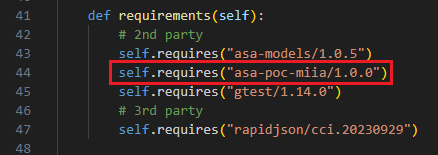
\includegraphics[width=0.72\textwidth]{images/conanfile.png}
    \caption{Declaração da dependência \texttt{asa-poc-miia/1.0.0} no \texttt{conanfile.py} do projeto cliente.}
    \label{fig:conanfile}
\end{figure}

Em seguida, carrega a dependência no \texttt{meson.build} raiz:

\vscodefile{meson.build}
\begin{lstlisting}[style=vscode]
asa_poc_miia_dep = dependency('asa-poc-miia')
\end{lstlisting}

\begin{figure}[h!]
    \centering
    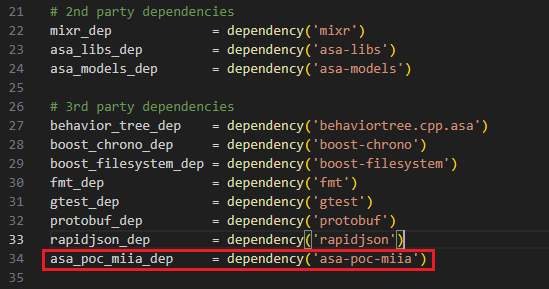
\includegraphics[width=0.82\textwidth]{images/meson root.png}
    \caption{Carregamento de \texttt{asa-poc-miia} como dependência no \texttt{meson.build} raiz do projeto cliente.}
    \label{fig:meson_root}
\end{figure}

E a vincula ao binário alvo no \texttt{src/meson.build}:

\vscodefile{src/meson.build}
\begin{lstlisting}[style=vscode]
executable('meu-projeto', sources, dependencies: [asa_poc_miia_dep])
\end{lstlisting}

\subsection{Uso no Código C++}

Com a dependência declarada, a integração no código C++ consiste em incluir o cabeçalho da biblioteca:

\begin{figure}[h!]
    \centering
    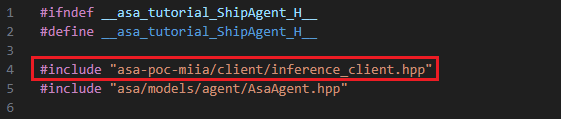
\includegraphics[width=0.72\textwidth]{images/include header.png}
    \caption{Inclusão do cabeçalho \texttt{asa-poc-miia/client/inference\_client.hpp} no \texttt{ShipAgent.hpp}.}
    \label{fig:include_header}
\end{figure}

Declarar o cliente e os atributos de estado na classe do agente:

\begin{figure}[h!]
    \centering
    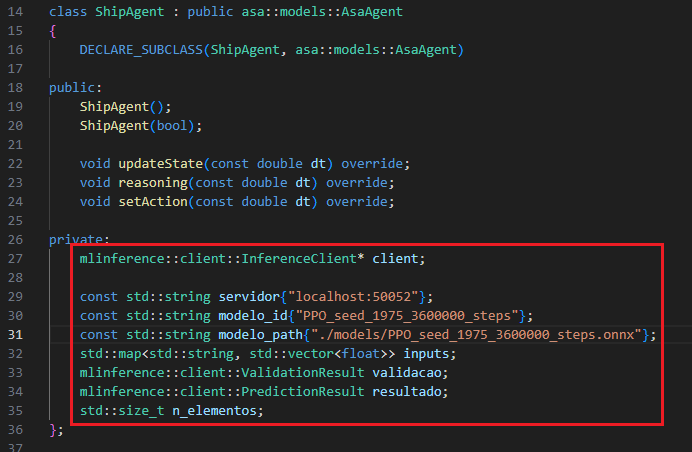
\includegraphics[width=0.72\textwidth]{images/class.png}
    \caption{Declaração do \texttt{InferenceClient} e dos atributos associados na classe \texttt{ShipAgent}.}
    \label{fig:class}
\end{figure}

Instanciar e inicializar o cliente no construtor:

\begin{figure}[h!]
    \centering
    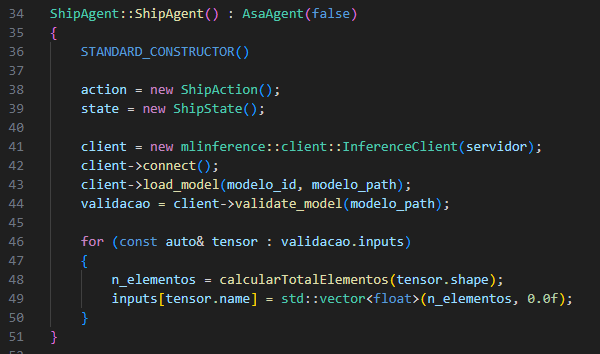
\includegraphics[width=0.72\textwidth]{images/contructor.png}
    \caption{Instanciação do \texttt{InferenceClient}, conexão e carregamento do modelo no construtor do \texttt{ShipAgent}.}
    \label{fig:constructor}
\end{figure}

E invocar a inferência no método de raciocínio do agente:

\begin{figure}[h!]
    \centering
    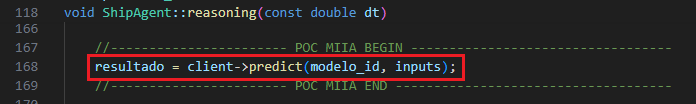
\includegraphics[width=0.82\textwidth]{images/inference.png}
    \caption{Chamada a \texttt{client->predict()} dentro do método \texttt{ShipAgent::reasoning()}.}
    \label{fig:inference}
\end{figure}

\section{Testes e Resultados}

\subsection{Cenário de Testes}

Os experimentos foram conduzidos utilizando o cenário \textbf{ASA Tutorial} (batalha naval --- Cel. Diego), executado em três condições distintas:

\begin{enumerate}
    \item \textbf{\textit{Status quo} (sem inferência)}: simulação rodando com comportamento original, sem qualquer chamada ao sistema de inferência. Utilizado como linha de base para comparação.

    \item \textbf{Inferência via servidor (\textit{client-server})}: a chamada de inferência é realizada a cada ciclo do laço de simulação, com um \textit{input} aleatório e resultado descartado. As decisões dos agentes permanecem as mesmas do \textit{status quo}. O objetivo é medir exclusivamente o impacto da chamada gRPC no desempenho da simulação.

    \item \textbf{Inferência \textit{in-process}}: a biblioteca cliente carrega o próprio modelo no mesmo processo do simulador, sem comunicação de rede, executando a inferência diretamente.
\end{enumerate}

\subsection{Resultados Obtidos}

A Tabela~\ref{tab:resultados} apresenta os valores de \textit{speedup} obtidos para cada condição na máquina de testes.

\begin{table}[h!]
\centering
% \begin{tabular}{|l|c|c|}
\begin{tabular}{|p{6cm}|c|c|}
\hline
\textbf{Condição} & \textbf{Speedup Máximo Prático} & \textbf{Variação em relação à base} \\
\hline
Sem inferência (\textit{status quo}) & 73,53$\times$ & --- \\
\hline
Com inferência --- cliente-servidor (gRPC) & 28,42$\times$ & $-$61,4\% \\
\hline
Com inferência --- \textit{in-process} & 44,44$\times$ & $-$39,6\% \\
\hline
\end{tabular}
\caption{Resultados de \textit{speedup} por condição de execução.}
\label{tab:resultados}
\end{table}

\begin{figure}[h!]
    \centering
    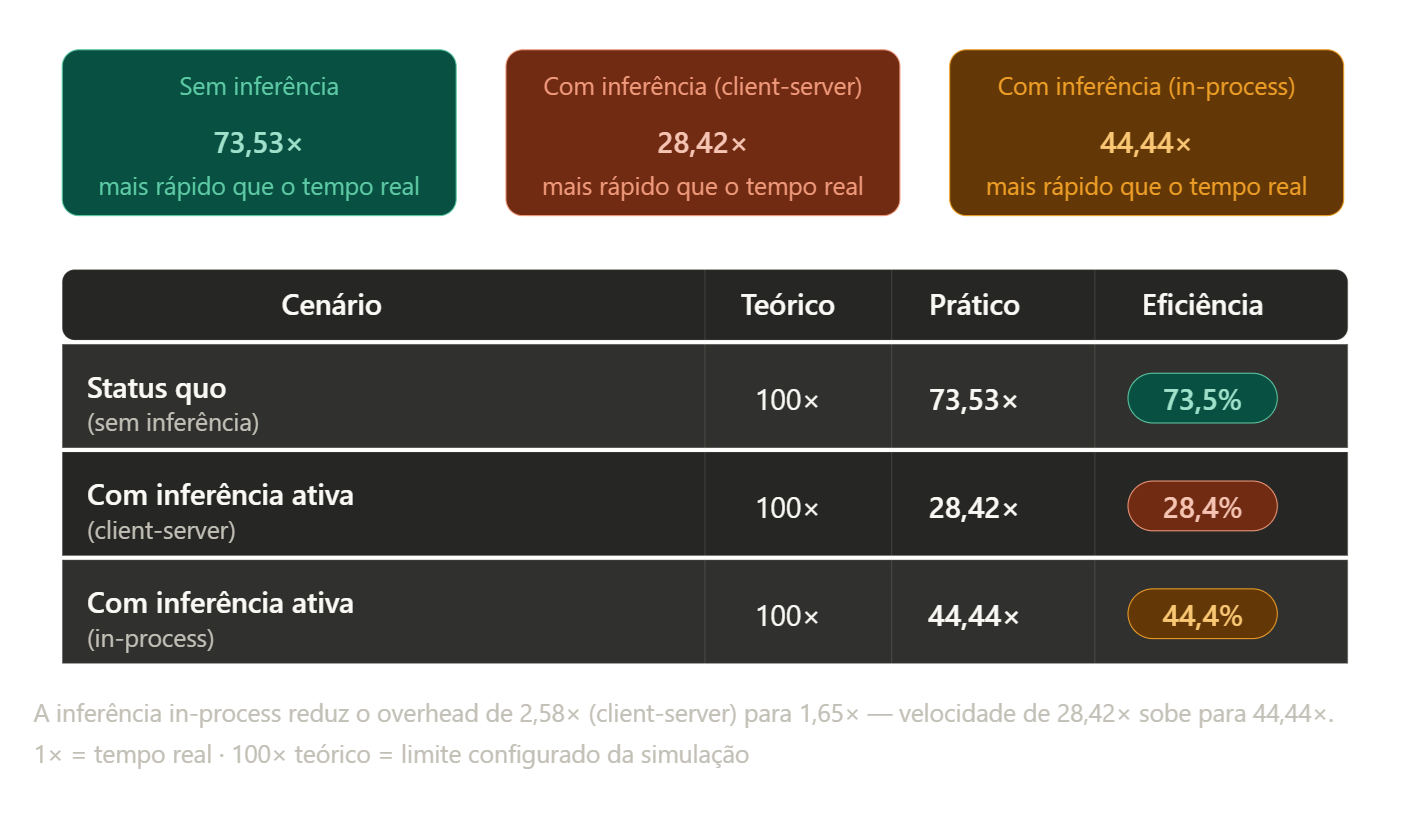
\includegraphics[width=\textwidth]{images/results.png}
    \caption{Comparativo visual dos resultados de speedup por cenário de execução.}
    \label{fig:results}
\end{figure}

\subsection{Análise dos Resultados}

Os resultados evidenciam que a comunicação gRPC representa o principal gargalo de desempenho: o modo cliente-servidor reduziu o \textit{speedup} em aproximadamente 61\% em relação à linha de base. Isso confirma que a latência de rede --- mesmo em comunicação local --- tem impacto significativo quando acionada em alta frequência dentro do laço de simulação.

A inferência \textit{in-process} apresentou desempenho intermediário, com redução de aproximadamente 40\% em relação à linha de base. Parte desse impacto é inerente à execução do modelo; o restante corresponde ao \textit{overhead} de interoperabilidade C++/Python ou do ONNX Runtime.

Ainda assim, ambos os modos mantiveram \textit{speedup} superior a 1$\times$, ou seja, a simulação continuou ocorrendo mais rápido que o tempo real, confirmando a viabilidade técnica da integração.

\section{Conclusões}

A PoC AsaMiia demonstrou ser tecnicamente viável a integração de inferência de ML ao laço de simulação do ASA/MIXR. A API unificada da biblioteca cliente simplifica a adoção por projetos existentes e futuros, abstraindo os detalhes do modo de execução escolhido.

O modo \textit{in-process} apresenta melhor desempenho e deve ser preferido em cenários onde a latência é crítica. O modo cliente-servidor, por sua vez, viabiliza o desacoplamento físico entre simulador e processo de inferência, permitindo o uso de hardware dedicado --- como GPU em servidor remoto --- sem alteração no código do agente.